%%%%%%%%%%%%%%%%%%%%%%%%%%%%%%%%%%%%%%%%%
% Short Sectioned Assignment LaTeX Template Version 1.0 (5/5/12)
% This template has been downloaded from: http://www.LaTeXTemplates.com
% Original author:  Frits Wenneker (http://www.howtotex.com)
% License: CC BY-NC-SA 3.0 (http://creativecommons.org/licenses/by-nc-sa/3.0/)
%%%%%%%%%%%%%%%%%%%%%%%%%%%%%%%%%%%%%%%%%

%----------------------------------------------------------------------------------------
%	PACKAGES AND OTHER DOCUMENT CONFIGURATIONS
%----------------------------------------------------------------------------------------

\documentclass[paper=a4, fontsize=11pt]{scrartcl} % A4 paper and 11pt font size

% ---- Entrada y salida de texto -----

\usepackage[T1]{fontenc} % Use 8-bit encoding that has 256 glyphs
\usepackage[utf8]{inputenc}
%\usepackage{fourier} % Use the Adobe Utopia font for the document - comment this line to return to the LaTeX default

% ---- Idioma --------

\usepackage[spanish, es-tabla]{babel} % Selecciona el español para palabras introducidas automáticamente, p.ej. "septiembre" en la fecha y especifica que se use la palabra Tabla en vez de Cuadro

% ---- Otros paquetes ----

\usepackage{url} % ,href} %para incluir URLs e hipervínculos dentro del texto (aunque hay que instalar href)
\usepackage{amsmath,amsfonts,amsthm} % Math packages
%\usepackage{graphics,graphicx, floatrow} %para incluir imágenes y notas en las imágenes
\usepackage{graphics,graphicx, float} %para incluir imágenes y colocarlas
\usepackage{epstopdf}

% Para hacer tablas comlejas
%\usepackage{multirow}
%\usepackage{threeparttable}

%\usepackage{sectsty} % Allows customizing section commands
%\allsectionsfont{\centering \normalfont\scshape} % Make all sections centered, the default font and small caps

\usepackage{fancyhdr} % Custom headers and footers
\pagestyle{fancyplain} % Makes all pages in the document conform to the custom headers and footers
\fancyhead{} % No page header - if you want one, create it in the same way as the footers below
\fancyfoot[L]{} % Empty left footer
\fancyfoot[C]{} % Empty center footer
\fancyfoot[R]{\thepage} % Page numbering for right footer
\renewcommand{\headrulewidth}{0pt} % Remove header underlines
\renewcommand{\footrulewidth}{0pt} % Remove footer underlines
\setlength{\headheight}{13.6pt} % Customize the height of the header

\numberwithin{equation}{section} % Number equations within sections (i.e. 1.1, 1.2, 2.1, 2.2 instead of 1, 2, 3, 4)
\numberwithin{figure}{section} % Number figures within sections (i.e. 1.1, 1.2, 2.1, 2.2 instead of 1, 2, 3, 4)
\numberwithin{table}{section} % Number tables within sections (i.e. 1.1, 1.2, 2.1, 2.2 instead of 1, 2, 3, 4)

\setlength\parindent{0pt} % Removes all indentation from paragraphs - comment this line for an assignment with lots of text

\newcommand{\horrule}[1]{\rule{\linewidth}{#1}} % Create horizontal rule command with 1 argument of height

\usepackage{listings}

%----------------------------------------------------------------------------------------
%	TÍTULO Y DATOS DEL ALUMNO
%----------------------------------------------------------------------------------------

\title{	
	\normalfont \normalsize 
	\textsc{\textbf{Curso 2016-2017} \\ Grado en Ingeniería Informática \\ Universidad de Granada} \\ [25pt] % Your university, school and/or department name(s)
	\horrule{0.5pt} \\[0.4cm] % Thin top horizontal rule
	\huge SPSI \\ Práctica 2: Protocolos criptográficos. \\ % The assignment title
	\horrule{2pt} \\[0.5cm] % Thick bottom horizontal rule
}

\author{Carlos Manuel Sequí Sánchez} % Nombre y apellidos

\date{\normalsize\today} % Incluye la fecha actual

%----------------------------------------------------------------------------------------
% DOCUMENTO
%----------------------------------------------------------------------------------------

\begin{document}
	
	\maketitle % Muestra el Título
	
	\newpage %inserta un salto de página
	
	\tableofcontents % para generar el índice de contenidos
	
	\listoffigures
	
	\newpage
	
	
	

%-------------------------------------------------------------------------------------

%-------------------------------------------------------------------------------------

%-------------------------------------------------------------------------------------

%-------------------------------------------------------------------------------------

%-------------------------------------------------------------------------------------

%-------------------------------------------------------------------------------------

%-------------------------------------------------------------------------------------

\section{EJERCICIO 1. Generad un archivo sharedDSA.pem que contenga los parámetros. Mostrad los valores. }

-Le especificamos el archivo de salida "sharedDSA.pem" y el numbits del archivo, ya que no le indicamos
ningún archivo de entrada: \\

\begin{lstlisting}
openssl dsaparam -out sharedDSA.pem 1024 \\
\end{lstlisting}

-Mostramos los valores en modo texto(hexadecimal), ya que en modo privado no se ve nada.
para ello hacemos uso del parámetro -text metiéndole como entrada el archivo de parámetros 
generado previamente y con la opción -noout para evitar que salga por pantalla el
archivo sharedDSA.pem. \\

openssl dsaparam -in sharedDSA.pem -text -noout

\begin{figure}[h]
	\centering
	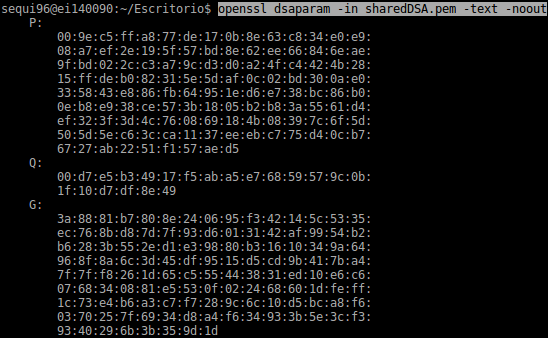
\includegraphics[width=0.9\textwidth]{imagenes/sharedDSA}
	\caption{sharedDSA.}
\end{figure}

\newpage

%-------------------------------------------------------------------------------------

%-------------------------------------------------------------------------------------

%-------------------------------------------------------------------------------------

%-------------------------------------------------------------------------------------

%-------------------------------------------------------------------------------------

%-------------------------------------------------------------------------------------

%-------------------------------------------------------------------------------------



\section{EJERCICIO 2. Generad dos parejas de claves para los parámetros anteriores. La claves se almacenarán en los archivos nombreDSAkey.pem y apellidoDSAkey.pem. No es necesario protegerlas por contraseña. }

-Generamos las dos parejas de claves a partir de los parámetros creados anteriormente: \\

openssl gendsa sharedDSA.pem -out CarlosDSAkey.pem 

openssl gendsa sharedDSA.pem -out SequiDSAkey.pem 



%-------------------------------------------------------------------------------------

%-------------------------------------------------------------------------------------

%-------------------------------------------------------------------------------------

%-------------------------------------------------------------------------------------

%-------------------------------------------------------------------------------------

%-------------------------------------------------------------------------------------

%-------------------------------------------------------------------------------------



\section{EJERCICIO 3. Extraed la clave privada contenida en el archivo nombreDSAkey.pem a otro archivo que tenga por nombre nombreDSApriv.pem. Este archivo deberá estar protegido por contraseña. Mostrad sus valores. Lo mismo para el archivo apellidoDSAkey.pem. }

-Extraemos las claves privadas con el comando "openssl dsa" utilizando los pares de claves generados en el ejercicio
anterior y, además, los ciframos con aes128 introduciéndoles como contraseña: 0123456789. \\

openssl dsa -in CarlosDSAkey.pem -aes128 -out CarlosDSApriv.pem\\

-Mostramos la clave:

openssl dsa -in CarlosDSApriv.pem -text -noout

\begin{figure}[h]
	\centering
	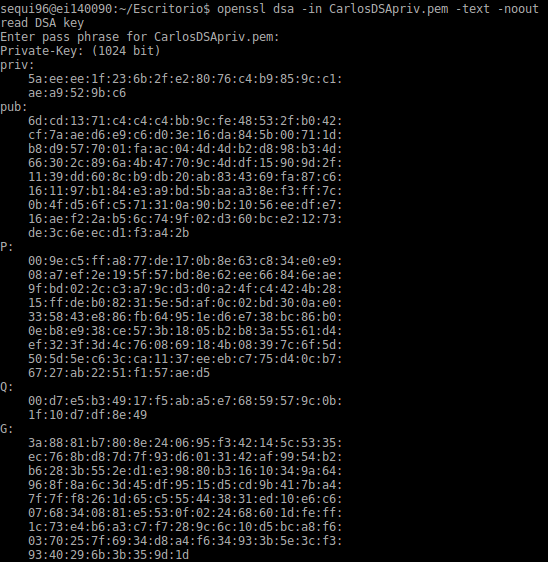
\includegraphics[width=0.9\textwidth]{imagenes/CarlosDSApriv}
	\caption{CarlosDSApriv.}
\end{figure}

\newpage

openssl dsa -in SequiDSAkey.pem -aes128 -out SequiDSApriv.pem \\

-Mostramos la clave:\\

openssl dsa -in SequiDSApriv.pem -text -noout

\begin{figure}[h]
	\centering
	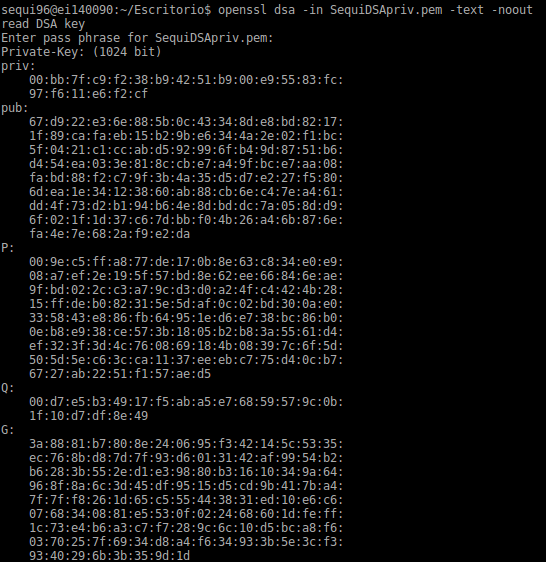
\includegraphics[width=0.9\textwidth]{imagenes/SequiDSApriv}
	\caption{SequiDSApriv.}
\end{figure}


%-------------------------------------------------------------------------------------

%-------------------------------------------------------------------------------------

%-------------------------------------------------------------------------------------

%-------------------------------------------------------------------------------------

%-------------------------------------------------------------------------------------

%-------------------------------------------------------------------------------------

%-------------------------------------------------------------------------------------


\section{EJERCICIO 4. Extraed en nombreDSApub.pem la clave pública contenida en el archivo nombreDSAkey.pem. De nuevo nombreDSApub.pem no debe estar cifrado ni protegido. Mostrad sus valores. Lo mismo para el archivo apellidoDSAkey.pem. }

-Extraemos las claves públicas con el comando "openssl dsa" utilizando los pares de claves generados en el ejercicio
anterior y, además, los ciframos con aes128 introduciéndoles como contraseña: 0123456789. \\

openssl dsa -in CarlosDSAkey.pem -out CarlosDSApub.pem -pubout\\

-Mostramos la clave:

openssl dsa -in CarlosDSApub.pem -text -noout -pubin

\begin{figure}[h]
	\centering
	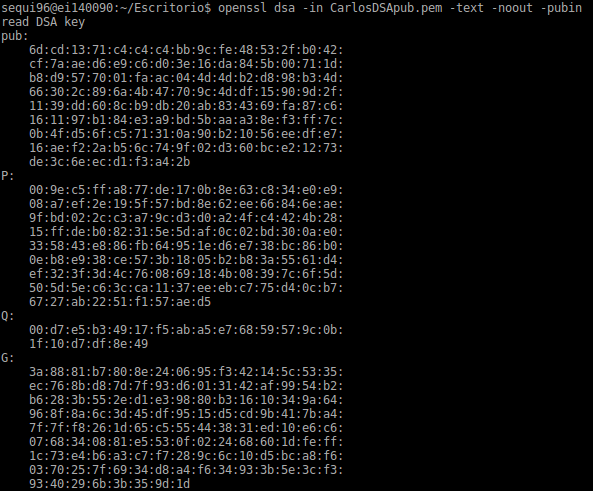
\includegraphics[width=0.9\textwidth]{imagenes/CarlosDSApub}
	\caption{CarlosDSApub.}
\end{figure}

openssl dsa -in SequiDSAkey.pem -out SequiDSApub.pem -pubout \\

-Mostramos la clave:\\

openssl dsa -in SequiDSApub.pem -text -noout -pubin

\begin{figure}[h]
	\centering
	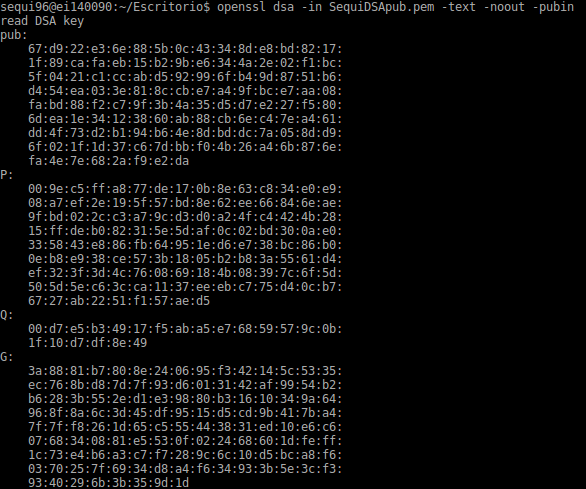
\includegraphics[width=0.9\textwidth]{imagenes/SequiDSApub}
	\caption{SequiDSApub.}
\end{figure}



%-------------------------------------------------------------------------------------

%-------------------------------------------------------------------------------------

%-------------------------------------------------------------------------------------

%-------------------------------------------------------------------------------------

%-------------------------------------------------------------------------------------

%-------------------------------------------------------------------------------------

%-------------------------------------------------------------------------------------


\section{EJERCICIO 5. Calculad el valor hash del archivo con la clave pública nombreDSApub.pem usando sha384 con salida hexadecinal con bloques de dos caracteres separados por dos puntos. Mostrad los valores por salida estándar y guardadlo en nombreDSApub.sha384.}

-Calculamos el valor hash usando sha384 con la salida hexadecimal (-hex) con bloques de dos caracteres separados por puntos (-c): \\

openssl dgst -sha384 -hex -c -out CarlosDSApub.sha384 CarlosDSApub.pem

-Mostramos dichos valores: \\

\begin{figure}[h]
	\centering
	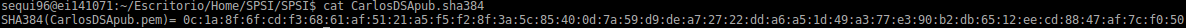
\includegraphics[width=1.2\textwidth]{imagenes/CarlosDSApubsha384}
	\caption{CarlosDSApub.sha384.}
\end{figure}


%-------------------------------------------------------------------------------------

%-------------------------------------------------------------------------------------

%-------------------------------------------------------------------------------------

%-------------------------------------------------------------------------------------

%-------------------------------------------------------------------------------------

%-------------------------------------------------------------------------------------

%-------------------------------------------------------------------------------------


\section{EJERCICIO 6. Calculad el valor hash del archivo con la clave pública apellidoDSApub.pem usando una función hash de 160 bits con salida binaria. Guardad el hash en apellidoDSApub.[algoritmo] y mostrad su contenido. }

-Usamos esta vez la salida binaria (-binary) con la función hash de 160 bits para el resumen del mensaje (-ripemd160):\\

openssl dgst -ripemd160 -binary -out SequiDSApub.ripemd160 SequiDSApub.pem \\

-Mostramos el contenido con la herramienta hexdump:\\

\begin{figure}[h]
	\centering
	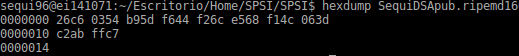
\includegraphics[width=1\textwidth]{imagenes/SequiDSApubripemd160}
	\caption{SequiDSApub.ripemd160.}
\end{figure}



%-------------------------------------------------------------------------------------

%-------------------------------------------------------------------------------------

%-------------------------------------------------------------------------------------

%-------------------------------------------------------------------------------------

%-------------------------------------------------------------------------------------

%-------------------------------------------------------------------------------------

%-------------------------------------------------------------------------------------


\section{EJERCICIO 7. Generad el valor HMAC del archivo sharedDSA.pem con clave ’12345’ mostrándolo por pantalla. }

-Generamos el valor HMAC de sharedDSA.pem con la clave '12345'

openssl dgst -hmac 12345 sharedDSA.pem

\begin{figure}[h]
	\centering
	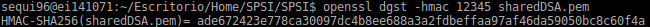
\includegraphics[width=1\textwidth]{imagenes/generacionHMAC}
	\caption{Valor HMAC de sharedDSA.pem.}
\end{figure}


%-------------------------------------------------------------------------------------

%-------------------------------------------------------------------------------------

%-------------------------------------------------------------------------------------

%-------------------------------------------------------------------------------------

%-------------------------------------------------------------------------------------

%-------------------------------------------------------------------------------------

%-------------------------------------------------------------------------------------


\section{EJERCICIO 8. Simulad una ejecución completa del protocolo Estación a Estación. Para ello emplearemos como claves para firma/verificación las generadas en esta práctica, y para el protocolo DH emplearemos las claves asociadas a curvas elípticas de la práctica anterior junto con las de otro usuario simulado que deberéis generar nuevamente. Por ejemplo, si mi clave privada está en javierECpriv.pem y la clave pública del otro usuario está en lobilloECpub.pem, el comando para generar la clave derivada será: \$> openssl pkeyutl -inkey javierECpriv.pem -peerkey lobilloECpub.pem -derive -out key.bin El algoritmo simétrico a utilizar en el protocolo}


-Una vez tenemos las claves firma/verificación generadas en esta práctica, procedemos a generar los pares de claves de curvas elípticas para
ambos usuarios a partir del mismo fichero de parámetros:

\begin{itemize}
	
	\item Para el usuario Carlos: \\
	
	openssl ecparam -in ./stdECparam.pem -genkey -noout -out ./CarlosECkey.pem 
	
	\item Para el usuario Sequi: \\
	
	openssl ecparam -in ./stdECparam.pem -genkey -noout -out ./SequiECkey.pem 
	
\end{itemize}

-Obtenemos para cada par de claves de curva elíptica de cada usuario, la privada y la pública:

\begin{itemize}
	\item SACAMOS LA PRIVADA:
	\begin{itemize}
		\item Para el usuario Carlos: \\
		
		openssl ec -in ./CarlosECkey.pem -out ./CarlosECpriv.pem -outform PEM -des3 
		
		\item Para el usuario Sequi: \\
		
		openssl ec -in ./SequiECkey.pem -out ./SequiECpriv.pem -outform PEM -des3 
	\end{itemize}
	\item SACAMOS LA PÚBLICA:
	\begin{itemize}
		\item Para el usuario Carlos: \\
		
		openssl ec -in ./CarlosECkey.pem -pubout -out ./CarlosECpub.pem
		
		\item Para el usuario Sequi: \\
		
		openssl ec -in ./SequiECkey.pem -pubout -out ./SequiECpub.pem
	\end{itemize}
\end{itemize}

-Derivamos las claves comunes a partir de las dos parejas privadaUsuario1/públicaUsuario2 (y viceversa) compartiendo parámetros.
Al compartir el mismo fichero de parámetros las claves de curvas elípticas, las claves que vamos a 
derivar ahora mismo serán exactamente iguales para Carlos y para Sequi.

\begin{itemize}
	\item La clave del usuario Carlos: \\
	
	openssl pkeyutl -inkey CarlosECpriv.pem -peerkey SequiECpub.pem -derive -out CarlosKey.bin
	
	\item La clave del usuario Sequi: \\
	
	openssl pkeyutl -inkey SequiECpriv.pem -peerkey CarlosECpub.pem -derive -out SequiKey.bin
\end{itemize}

-Cada usuario concatena su clave pública de la curva elíptica con la clave pública de la curva elíptica que ha 
recibido por parte del otro usuario y, utiliza una concatenación para firmar y otra para verificar a identidad del otro usuario:

\begin{itemize}
	\item Fichero concatenado del usuario Carlos: \\
	\begin{itemize}
		\item Para firmar: cat CarlosECpub.pem SequiECpub.pem > ficheroConcatenadoFirmarCarlos
		\item Para verificar: cat SequiECpub.pem CarlosECpub.pem > ficheroConcatenadoVerificarCarlos
	\end{itemize}
	
	\item Fichero concatenado del usuario Sequi: \\
	\begin{itemize}
		\item Para verificar: cat CarlosECpub.pem SequiECpub.pem > ficheroConcatenadoVerificarSequi
		\item Para firmar: cat SequiECpub.pem CarlosECpub.pem > ficheroConcatenadoFirmarSequi
	\end{itemize}
	
\end{itemize}

-Cada usuario firma el fichero concatenado obtenido

\begin{itemize}
	\item Firma por parte del usuario Carlos: \\
	
	openssl dgst -sha256 -sign ./CarlosDSApriv.pem -out ./ficheroFirmadoCarlos.sha256 ./ficheroConcatenadoFirmarCarlos
	
	\item Firma por parte del usuario Sequi: \\
	
	openssl dgst -sha256 -sign ./SequiDSApriv.pem -out ./ficheroFirmadoSequi.sha256 ./ficheroConcatenadoFirmarSequi
\end{itemize}

-Cada uno de los usuarios procede a encriptar el fichero firmado con AES-128 en modo CFB8 usando la clave derivada:

\begin{itemize}
	\item Encriptación en AES-128 modo CDB8 por parte del usuario Carlos: \\
	
	openssl enc -aes-128-cfb8 -pass file:./CarlosKey.bin -in ficheroFirmadoCarlos.sha256 -out ficheroFirmadoEncriptadoCarlos.bin
	
	\item Encriptación en AES-128 modo CDB8 por parte del usuario Sequi: \\
	
	openssl enc -aes-128-cfb8 -pass file:./SequiKey.bin -in ficheroFirmadoSequi.sha256 -out ficheroFirmadoEncriptadoSequi.bin
\end{itemize}

-Los usuarios reciben los correspondientes ficheros firmados y después encriptados por parte del otro usuario y, proceden a desencriptarlo
primeramente usando la clave derivada que, como hemos dicho, son iguales para ambos usuarios:

\begin{itemize}
	\item Desencriptación en AES-128 modo CDB8 por parte del usuario Carlos: \\
	
	openssl aes-128-cfb8 -d -pass file:./CarlosKey.bin -in ficheroFirmadoEncriptadoSequi.bin -out ./ficheroFirmadoDesencriptadoPorCarlos.sha256
	
	\item Desencriptación en AES-128 modo CDB8 por parte del usuario Sequi: \\
	
	openssl aes-128-cfb8 -d -pass file:./SequiKey.bin -in ficheroFirmadoEncriptadoCarlos.bin -out ./ficheroFirmadoDesencriptadoPorSequi.sha256
\end{itemize}

-Ahora proceden a la verificación para asegurarse de la comunicación es entre los usuarios que han de ser.
El usuario1, para verificar el fichero, utiliza la clave pública que le manda el usuario2 y verifica usando el fichero que ha desencriptado (que previamente e habia mandado el usuario2) y su propio fichero concatenado, el que había creado él mismo antes.

\begin{itemize}
	\item Verificación por parte del usuario Carlos: \\
	
	openssl dgst -verify SequiDSApub.pem -signature ./ficheroFirmadoDesencriptadoPorCarlos.sha256 ficheroConcatenadoVerificarCarlos
	
	\item Verificación por parte del usuario Sequi: \\
	
	openssl dgst -verify CarlosDSApub.pem -signature ./ficheroFirmadoDesencriptadoPorSequi.sha256 ficheroConcatenadoVerificarCarlos
\end{itemize}

-Obtenemos un "Verified OK" por terminal en caso de que la verificación haya sido correcta (en caso contrario un "Verification Failure").

\begin{figure}[h]
	\centering
	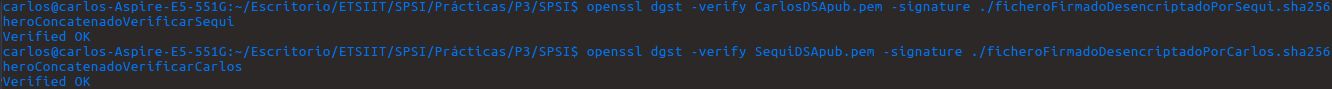
\includegraphics[width=1.2\textwidth]{imagenes/verificacion}
	\caption{Muestra de la correcta verificación de ambos archivos}
\end{figure}



%-------------------------------------------------------------------------------------

%-------------------------------------------------------------------------------------

%-------------------------------------------------------------------------------------

%-------------------------------------------------------------------------------------

%-------------------------------------------------------------------------------------

%-------------------------------------------------------------------------------------

%-------------------------------------------------------------------------------------







\newpage
%------------------------------------------------

\bibliography{citas} %archivo citas.bib que contiene las entradas 
\bibliographystyle{plain} % hay varias formas de citar




\end{document}
